\documentclass[12pt]{report}
\pagestyle{headings}

\usepackage[pdftex]{graphicx}
\usepackage[tt]{titlepic}
\usepackage[latin1]{inputenc}
\usepackage[T1]{fontenc}

\setlength{\parindent}{0.0in}
%\setlength{\parskip}{0.1in}
\setcounter{secnumdepth}{-1}
\setcounter{tocdepth}{1}

%\addtolength{\textheight}{2cm}
%\addtolength{\footskip}{2cm}

\renewcommand*\contentsname{Innhold}
\renewcommand*\listtablename{Tabell-liste}
\renewcommand*\listfigurename{Figurliste}
\renewcommand*\chaptername{Kapittel}
\renewcommand*\partname{Del}
\renewcommand*\figurename{Figur}
\renewcommand*\tablename{Tabell}

\newcommand\placeholder[2]{
	\noindent
	{\setlength{\fboxsep}{0pt}
		\makebox[#1]{
			\parbox{0pt}{\rule{0pt}{#2}}
			\parbox{#1}{
				\centering
				
\includegraphics[width=0.50\textwidth]{graphics/logo.png}
			}
		}
	}
}

\titlepic{\placeholder{\textwidth}{0.5\textwidth}}
\title{{\Large Eksperter i Team\\TPG4850 VR-Landsbyen\\{\bf Virtual Insanity (Team 4)\\Fagrapport}}}
\author{Holger Ludvigsen,\\Vegar Neshaug,\\Rahele Zarabi,\\Jon Skarpetveit,\\Kristoffer Selboe}
\date{{\small \today}}

\begin{document}
\maketitle

\chapter{Summary of report}
	As a part of the course Experts in Team (EiT) at NTNU, five students were put in a group to collaborate on a project. This team (us) was a part of the virtual reality village of EiT, and came up with the following problem statement:

\begin{center}\em How can you make an affordable and usable prototype\\for head tracking to be used for virtual reality?\end{center}
\vspace{\parskip}

We solved this problem by first doing a preliminary study followed by design and imlementation of the solution. In the preliminary study, several technical and theoretical subjects were investigated. The mathematics behind estimation of object position from pictures were elaborated. We looked at the available technology for connecting a high definition camera to a PC and reading the images from it. We studied the properties of infrared light. We checked out and tested the Nintendo Wii and its Wiimotes. Lastly, potential areas of use for a solution was described.

Then, a specification of the requirements was carefully crafted. The specification was the basis for the design of the solution. This design specifies how the components of the system is constructed and how they are connected. The components of the system make up a pipeline:

\begin{figure}[h]
\centering
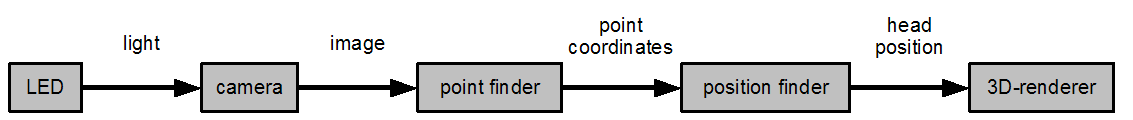
\includegraphics[width=\textwidth]{graphics/main_design_english.png}
\end{figure}

The LED-component is a set of infra red LEDs that are attached to the user's head. These transmit light that is captured by a high definition camera. The image from this camera is read by a point finder software that attempts to locate the coordinates of the bright dots in the image where the LEDs are. These coordinates are transferred to the position finder software which uses them to estimate the position of the user's head. This head position is then used by the 3D-renderer software to display a 3D-scene on a screen where the viewpoint is mapped to the head position.

Course
Project group
Problem statement
Prestudy
How solved:
	Reqspec
	Design
	Implementation
Result
Evaluation
Conclusion
\pagebreak
	
\setlength{\parskip}{0.0in}
\tableofcontents
%\listoftables
%\listoffigures
%\pagebreak
\setlength{\parskip}{0.1in}

\chapter{Innledning}

	\chapter*{Introduksjon}

\chapter{Forstudie}

	\section{Matematikken bak trackingen (Vegar)}

	

\section{Tilkobling av kamera til PC}

	For � koble et kamera til en PC og lese dens videobilder trenger man b�de maskinvare og programvare. Maskinvaren gir den fysiske tilkoblingen mellom kameraet og PC-en samt gj�r lavniv�s logikk og behandling av dataene. Programvaren abstraherer bort maskinvaren og gir utviklere et brukbart grensesnitt for � lese og bruke videobildene. Av maskinvare har vi i prosjektet tenkt � bruke HDMI og et Intensity-kort for � koble kameraet til PC-en som kj�rer systemet v�rt. Av programvare har vi tenkt � bruke DirectShow for � f� lett tilgang til videobildene fra kameraet.
	
\subsection{HDMI og Intensity}

	HDMI er en standard for et fysisk grensesnitt for � sende og motta digital lyd og bilde. Apparater med HDMI-kontakt kan kobles til hverandre ved hjelp av en HDMI-kabel (se figur \ref{fig:hdmi}). HDMI er designet for � h�ndtere lyd og bilde med h�y oppl�sning, og kan sende opptil 10,2 gigabit per sekund.
	
	\begin{figure}[h]
	\centering
	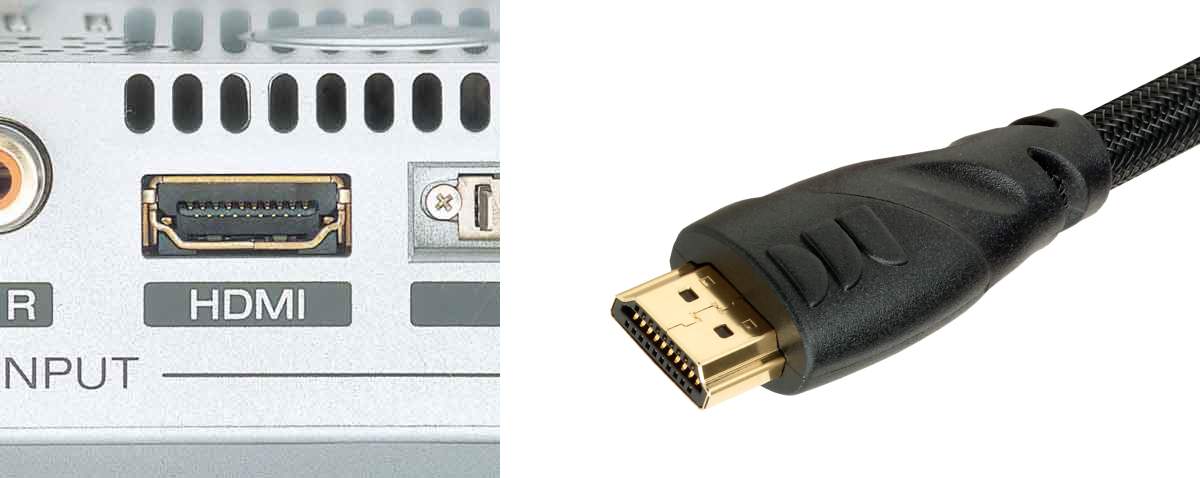
\includegraphics[width=0.60\textwidth]{graphics/hdmi.png}
	\caption{HDMI-kontakt (venstre) og kabel (h�yre)}
	\label{fig:hdmi}
	\end{figure}
	
	Intensity er et HDMI capture card fra Blackmagic Design. Det er et stykke maskinvare som kan settes inn i en PC for � gj�re det mulig � koble enheter til denne PC-en gjennom HDMI. Kortet kobles til PCI-express-porten i PC-en og har to HDMI-kontaktpunkter: inngang og utgang (se figur \ref{fig:intensity}).
	
	For � kunne f� ut bilde fra HD kameraet trengte vi HDMI input port som overf�rer data i en s� stor hastighet slik at vi slipper � komprimere bildestr�mmen. Vi valgte Blackmagic Intesity card som gir den beste og siste teknologien innen HDMI til Windows eller Mac OS. Intesity kortet har en HDMI inngang for HD kameraer som gir den h�yeste kvalitet p� bilde. HDMI kan lese ukomprimert bildestr�m direkte fra kameraet. Bildestr�mmen er i 1080i (interlaced) det vil si at bilde har en oppl�sning p� 1920 x 1080 piksler. 1080 linjer i vertikal retning og 1920 linjer i horisontal retning. Interlaced betyr at kameraet tar opp bilder med et alternerende sett med linjer slik at oddetallslinjene og partallslinjene oppdateres annenhver gang. Det vil si at det trengs to oppdateringer for � skape et fullstendig bilde, man �ker bildekvaliteten av et videosignal uten � �ke b�ndbredden. N�r bildet skal vises p� skjerm utf�res det en deinterlacing som er en teknikk for � konvertere interlaced bildestr�m til progressive bildestr�m. Hvis det er 1080p (progressive) trenger bildestr�mmen kun � oppdateres en gang for � f� et fullstendig bilde, at alle linjene vertikalt blir skannet ved en oppdatering. 
	 
	\begin{figure}[h]
	\centering
	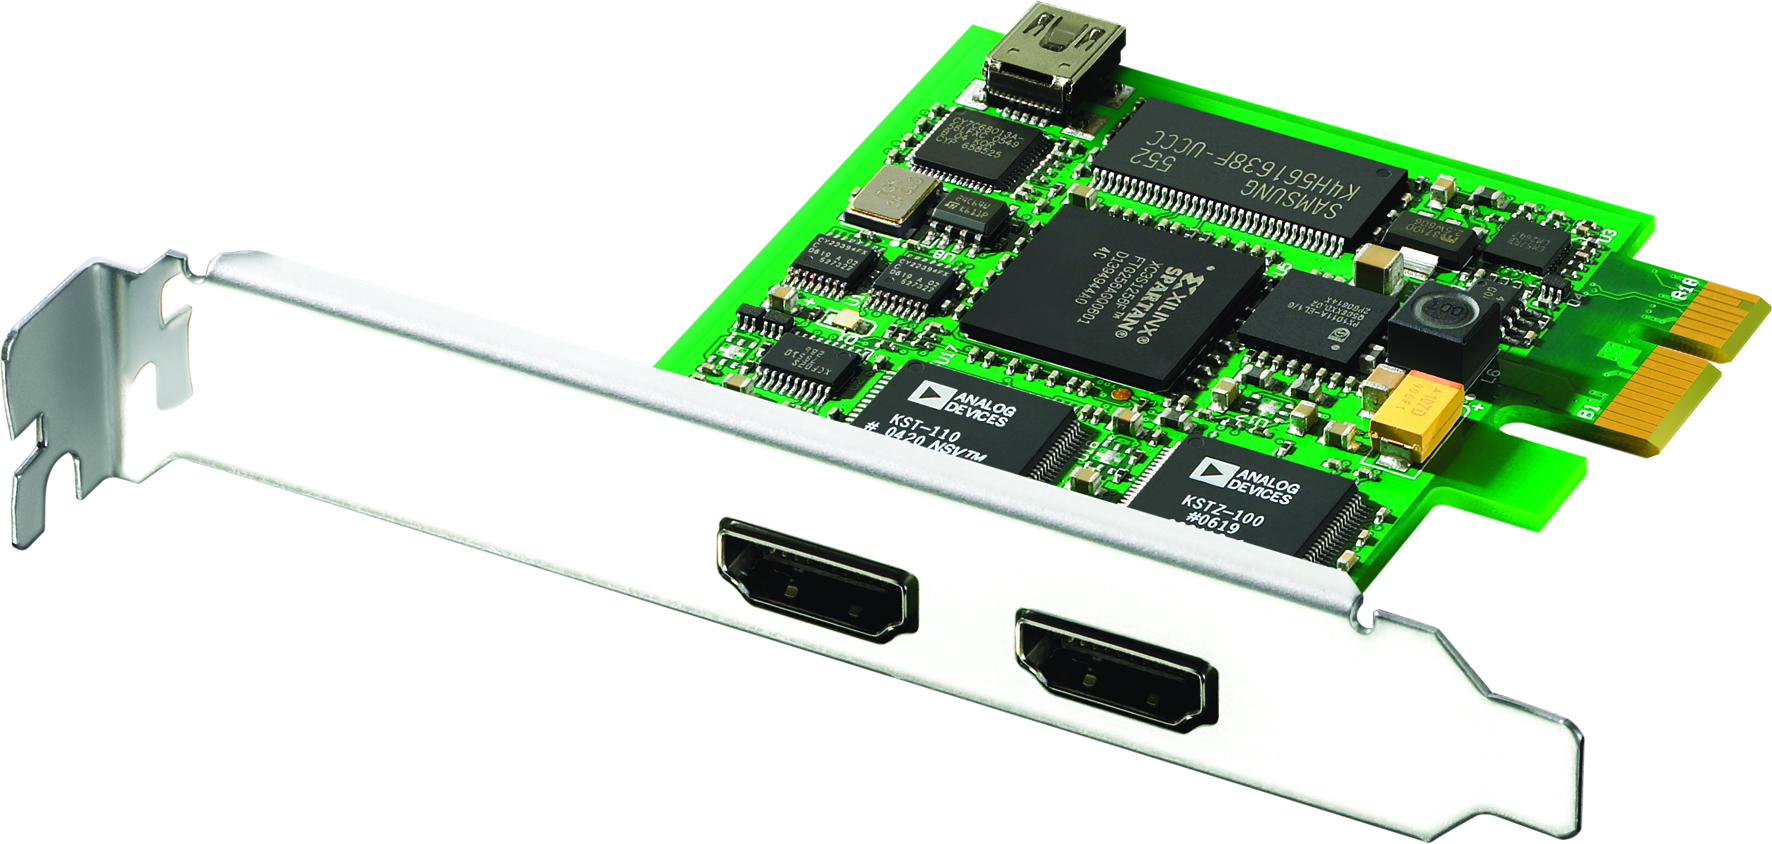
\includegraphics[width=0.60\textwidth]{graphics/intensity.png}
	\caption{Intensity fra Blackmagic Design}
	\label{fig:intensity}
	\end{figure}

\subsection{DirectShow}

	DirectShow er et rammeverk og programvaregrensesnitt for � h�ndtere multimedia p� PC-er. Det er utviklet av Microsoft og gj�r det mulig � spille av og ta opp media (typisk lyd og/eller bilde) gjennom et felles grensesnitt, og abstraherer bort maskinvaren. Bildene fra videokamera koblet til et Intensity-kort er tilgjengelig gjennom DirectShow. DirectShow er tilgjengelig gratis fra Microsofts nettsider.
	
\subsection{Infrar�dt lys}

	Infrar�d lys er elekektromagnetisk str�ling av b�lgelengder lengre enn b�lgelengdene til synlig lys. Det synlige lyset har b�lgelengder mindre enn 750nm. Ordet infra kommer fra latinsk og betyr under, og r�d er den fargen innenfor det synlige spekteret som har den lengste b�lgelengden. Det infrar�de lyset som ligger n�rmest det synlige lys har mye av de samme egnskapene som det synlige lyset bortsett fra at det er usynlig for det mennesklige �yet. Infrar�dtlys er derfor mye brukt til blant annet overv�kning og nattkamera, i tillegg til ignaler i elektriske kontroller. Infrar�d str�ling med lengre b�lgelengder er mer knyttet til varmeproduksjon og varmesensitive kameraer som er mye brukt i romfartsindustri og v�penindustri.

	I dette prosjektet er det en fordel � bruke infrar�dt lys fordi et lyspunkt som er synlig for det mennesklige �yet kan v�re forstyrrende for brukeren og det kan blande seg med andre lyskilder i omgivelsene rundt som vil gj�re det vanskligere finne punktene vi �nsker under prosesseringsarbeidet. 
	
\section{Nintendo Wii og Wiimotes}

	Nintendo Wii er en spillkonsoll som ble lansert i 2006. I stedet for realistisk grafikk fokuserer den p� alternative former for styring av spill. Wiimote er navnet p� kontrolleren som brukes for Wii. Se figur \ref{fig:wiimote}. Det er en tr�dl�s kontroller med infrar�dt kamera og akselerasjonsmeter. Innebygd er det maskinvare som kalkulerer bildekoordinater til filmede infrar�de lys og sender disse via et tr�dl�st nettverk (Bluetooth).
	
	\begin{figure}[h]
	\centering
	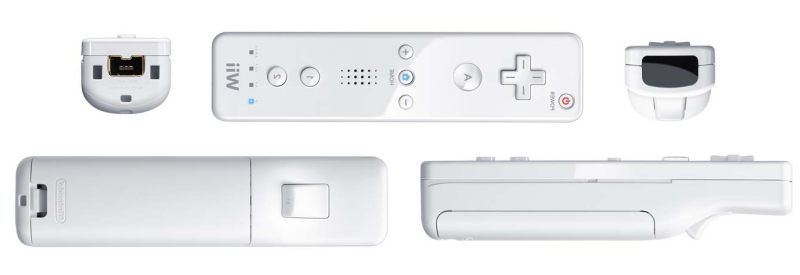
\includegraphics[width=0.60\textwidth]{graphics/wiimote.png}
	\caption{Nintendo Wiimote}
	\label{fig:wiimote}
	\end{figure}

\section{� spore punkter i et bilde (Holger)}

	

\section{Bruksomr�der (Jon)}

	

\chapter{Kravspesifikasjon}

		I dette kapitlet spesifiseres kravene til systemet som skal utvikles. Kravene er delt inn i funksjonelle og ikke-funksjonelle krav. Funksjonelle krav beskriver hva et system er i stand til � gj�re. De spesifiserer ikke kvaliteten, effektiviteten eller implementasjonen av disse funksjonene. Med andre ord, the sier \emph{hva} en bruker kan gj�re med systemet. Ikke-funksjonelle krav beskriver egenskaper ved systemet som ikke er direkte funksjoner. De er relatert til systemet som en helhet. Tabell \ref{table:f_req_spec} og \ref{table:nf_req_spec} viser de funksjonelle og ikke-funksjonelle kravene til systemet som skal lages.
	
	\begin{table}[h]
		\centering
		\begin{tabular}{| c | c | p{9 cm} |}
			\hline 
			\bf ID & \bf Prior. & \bf Description \\
			\hline
			\hline
			FR1 & H�y & Systemet skal spore posisjonen til et menneskehode i tre dimensjoner. \\
			FR2 & H�y & Den sporede posisjonen skal oppdateres n�r hodet beveger p� seg. \\
			FR3 & Lav & En tre-dimensjonal scene skal vises p� en skjerm foran menneskehodet hvor kameraposisjonen i scenen er lik posisjonen til hodet i rommet. \\
			\hline
		\end{tabular}
		\caption{Funksjonelle krav}
		\label{table:f_req_spec}
	\end{table}
	
	\begin{table}[h]
		\centering
		\begin{tabular}{| c | c | p{9 cm} |}
			\hline 
			\bf ID & \bf Prior. & \bf Description \\
			\hline
			\hline
			NFR1 & H�y & Prisen for systemet skal v�re under 10 000 NOK. \\
			NFR2 & Lav & Eventuelt utstyr brukeren m� ha p� seg skal v�re lettere enn 300 gram. \\
			\hline
		\end{tabular}
		\caption{Ikke-funksjonelle krav}
		\label{table:nf_req_spec}
	\end{table}
	
\chapter{Design og implementasjon}

	\section{Design av l\o sningen}

	

\section{Implementasjon av l\o sningen}

	

\chapter{Resultat}

	\section{Hva prosjektet endte opp med}

	Etter implementasjonen endte vi opp med en adaptiv l�sning. I tillegg til � kunne bruke HD-kameraet kan det brukes Nintendo Wiimotes. Systemet tilbyr virtuell virkelighet etter kravspesifikasjonen, og st�tter f�lgende konfigurasjoner:
	
	\begin{itemize}
		\item Et HD-kamera som filmer to lys p� hodet
		\item En Wiimote som filmer to lys p� hodet
		\item To Wiimotes som filmer ett lys p� hodet
	\end{itemize}
	
	Felles for alle er at et eller flere kamera (Wiimote eller HD-kamera) filmer lys montert p� hodet. Programvaren bruker disse bildene til � estimere posisjonen til hodet i rommet.
	
	\begin{description}
		\item[Et HD-kamera som filmer to lys p� hodet] Her er det et HD-kamera som filmer to infrar�de LEDs p� hodet til brukeren. I denne konfigurasjonen f�lger systemet designen beskrevet i designseksjonen over til punkt og prikke.
		\item[En Wiimote som filmer to lys p� hodet] I denne konfigurasjonen er HD-kameraet byttet ut med en Nintendo Wiimote som ogs� tar seg av � finne koordinatene til lyspunktene i bildet som filmes. Disse koordinatene sendes tr�dl�st til v�r programvare hvor de brukes til � beregne hodeposisjon og vise en 3D-scene akkurat som i konfigurasjonen over.
		\item[To Wiimotes som filmer ett lys p� hodet] I denne konfigurasjonen brukes {\em to} Wiimotes. Dette betyr at kun ett lys trengs p� hodet.
	\end{description}

    \subsection{Demonstrasjonsprogrammer}
    En av m�lsetningene til prosjektgruppa var � produsere en eller flere demonstrasjonsprogrammer
    som viser hvordan hodetracking kan brukes.
    \subsubsection{Illusjonen}
        \begin{figure}[h]
	\centering
	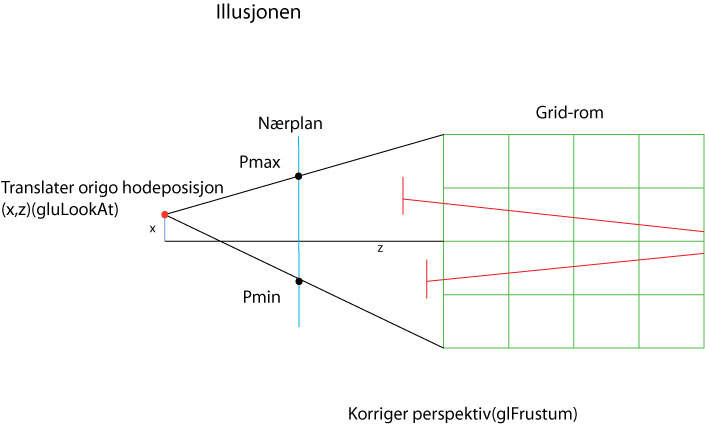
\includegraphics[width=0.80\textwidth]{graphics/Illusjonen.jpg}
	\caption{Illustrasjon illusjon}
	\label{fig:illusjon}
	\end{figure}
    Johnny Chung demonstrerer i en video p� youtube
    hvordan man kan f� et objekt til � tilsynelatende bryte skjermflaten og sveve ut i rommet foran skjermen.
    Denne illusjonen ble gjenskapt i produktet. Hvordan denne effekten oppst�r kan kanskje en psykolog forklare
    best, men rent teknisk oppn�s denne effekten ved � angi dybden til n�rplanet/klippeplanet, som n�rmere enn
    starten p� grid-rommet og benytte en perspektivprojeksjonen som gj�r at grid-rommet er kant-i-kant med skjermen.
    Et objekt som befinner seg lenger frem enn skjermkantene vil da likevel tegnes p� grunn av et n�rmere n�rplan.
    I demonstrasjonen tegnes en linje fra bakveggen i rommet til objektet, sammenligner man denne linjen med linjene
    i grid-rommet vil man se at linjen til objektet later til � v�re lenger, og dette forsterker inntrykket av at
    objektet er lenger ut i rommet enn skjermflaten. 
    F�lgende ligninger brukes for � regne ut et n�rmere n�rplan. Se ogs� figur \ref{fig:illusjon}.
    Definer $d$ som dybden til �nsket n�rplan.

	
    \begin{eqnarray}
    &p_{min} = d\frac{b-x}{z}\\
    &p_{max} = d\frac{a-x}{z}
    \end{eqnarray}
    For y-aksen gjelder figur og ligninger med x utbyttet med y.


	
	\subsubsection{Spillet}
	For � f� en engasjerende og morsom demonstrasjon valgte vi � implementere et spill som best�r av et virtuelt rom
	hvor forskjellige gjenstander beveger seg mot spilleren. Dette kan sammenlignes med TV-underholdningsprogrammet "Ylvis m�ter veggen"
	hvor deltagerne pr�ver � komme seg igjennom en form i en vegg. Hodetracking gir oss en indikasjon p� hvor spilleren befinner seg,
	dette kan brukes til � bestemme om spilleren kolliderer med eller unng�r solide objekter. Spilleren m� hoppe over, dukke under og
	l�pe til siden av objekter for � unng� kollisjon. Poengsummen bestemmes av hvor lenge spilleren har klart � unng�
	objektene, som kommer flyvende imot b�de i �kende antall og med �kende hastighet. Dette gir et meget godt bilde p�
	hvordan et spill blir mer engasjerende n�r spilleren ikke sitter tiln�rmet passiv i godstolen, men m� opp og r�re p� seg
	for � f� en god score.


\section{Evaluering av resultatet}
	
	L�sningen vi endte opp med f�lger kravspesifikasjonene og designen. Den estimerer posisjonen til hodet ved � filme infrar�de LEDs montert p� hodet, og bruker denne til � skape en virtuell virkelighet p� skjermen foran brukeren. Vi starter evaluering ved � p�peke svakhetene ved systemet, og avslutter med styrkene.
	
	\subsection{Svakheter ved systemet}
		\subsubsection{HD-kameraet har forsinkelse}
		
			N�r systemet endelig var kapabelt til � motta bilder fra HD-kameraet og spore lyspunktene ble det klart at det er forsinkelse p� disse bildene. Denne forsinkelsen er ca 0,5 sekunder og er i stor grad merkbar. Vi h�pet tidligere at forsinkelsen var en eller annen flaskehals som bare eksisterte i den tidlige suboptimale koden vi brukte for � f� ting til � fungere, men det ser ut til at dette er en iboende egenskap ved HD-kameraet og/eller overf�ringen av bildene gjennom HDMI-kortet. Siden kameraet har h�y oppl�sning er det mange piksler som skal sendes. I tillegg til dette er kameraet ikke beregnet for sanntidsfilming, men heller � ta opp for � se senere. Heldigvis er Wiimotesene beregnet p� denne bruken og har neglisjerbar forsinkelse.
		
		\subsubsection{LED-headsettet er ikke profesjonelt}
		I forhold til Nintendo sensorbar er ikke headsettet en like god lyskilde.
		Nintendo senorbare har en vifteform av LED's samt en skikkelig lysspreder(diffusjonsglass).
		
		Selv om det for prosjektgruppa er sjarmerende med et headsett som har synlige r�de og sorte
		ledninger, med kledelig sort elektrikerteip, er dette ikke like betryggende for de personene som tester systemet.
			
	
	\subsection{Styrker ved systemet}
	
		\subsubsection{HD-kamera har h�y oppl�sning}
		
			HD-kameraets h�ye oppl�sning gj�r at sm� LEDs synes p� lang avstand. Dette betyr at man kan st� langt unna kameraet, og dermed ogs� langt unna skjermen, og fortsatt oppleve god respons p� hodebevegelser. Aberet er at h�yere oppl�sning betyr flere piksler � prosessere i s�k etter lysprikkene, men dette ser ikke ut til � v�re den st�rste flaskehalsen med de n�v�rende algoritmene.
		
		
			
		
		\subsubsection{Virkelighetsf�lelsen er sterk}
		
			Det finnes mange ulike systemer for virtuell virkelighet. Virkemidlene de bruker for � oppn� denne illusjonen varierer sterkt, og ingen dekker alle sansene p� en gang. V�rt system simulerer virkningene av � bevege hodet n�r man ser p� noe. Dette gir en sterk virkelighetsf�lelse fordi hjernen kobler sammen hvordan kroppen beveger seg med hva den ser. For at hjernen skal tro at den ser p� et 3-dimensjonal objekt m� synet matche bevegelsene, og det gj�r de i v�rt system.
	 \subsection{Testresultater}
    For � f� et inntrykk av n�yaktigheten til posisjoneringen merket vi opp avstander i et rom, kalibrerte program og utstyr og
    foretok m�linger p� de oppmerkede punktene.
    
    F�lgende tabell viser n�yaktigheten til systemet ved bruk av henholdsvis en sensor(kuleskallmodell) og to sensorer(triangulering).
    
    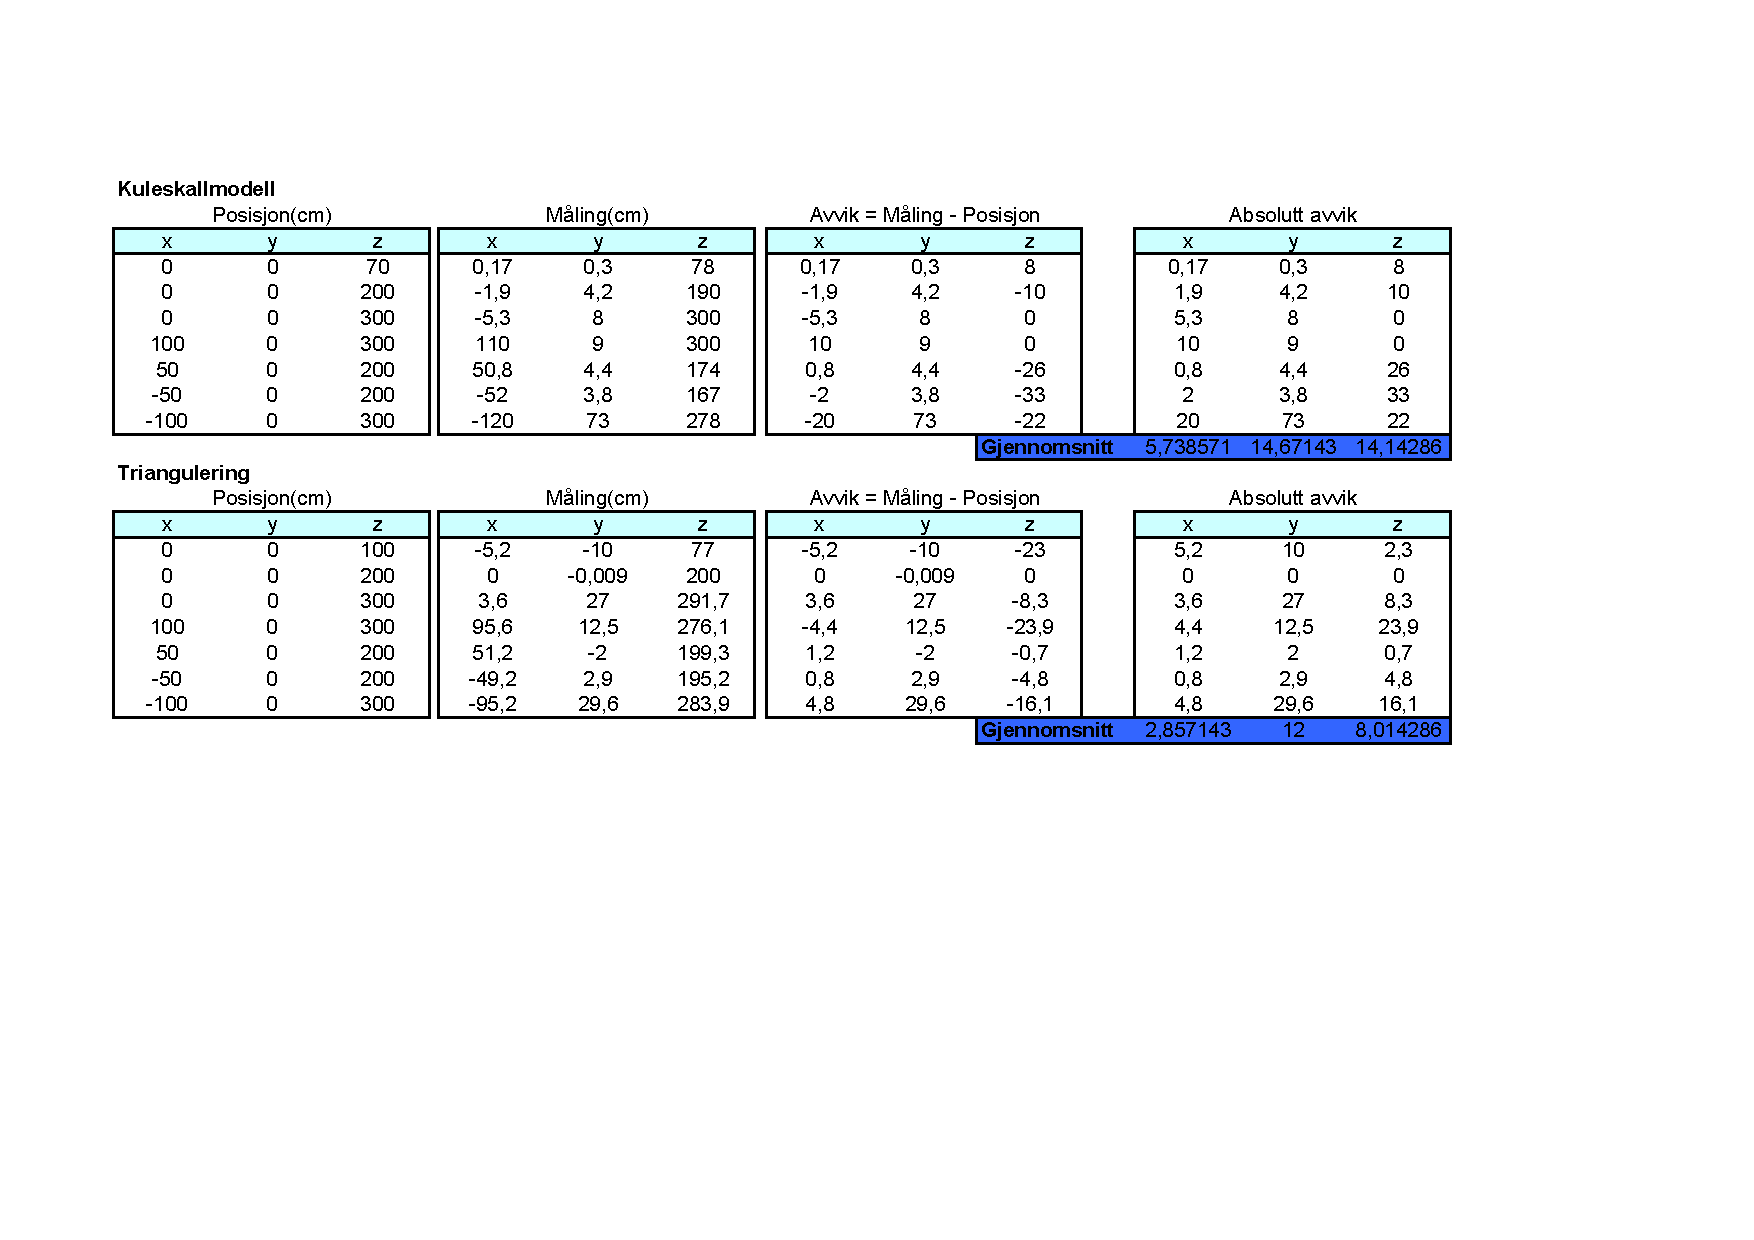
\includegraphics[width=1.25\textwidth]{graphics/testresults.pdf}
    
    \addtolength{\parskip}{-1in}
    
    F�lgende feilkilder m� tas med i tolkningen av resultatet.
    \begin{enumerate}
    \item Avstandsoppmerkingen ble gjort med tommestokk, og er n�yaktig innenfor et par centimeter.
    \item Ved bruk av en sensor, er det ikke alltid at hodet er vendt n�yaktig vinkelrett p� sensor, slik som modellen antar.
    \item M�lepunktene med stor x-verdi er veldig n�rt maksimal utsynsvinkel for sensor.
    \end{enumerate}
    
    \addtolength{\parskip}{1in}
	
	Det mest �penbare resultatet er at gjennomsnittlig absolutt avvik er mindre ved bruk av triangulering. 
	Det er verdt � merke seg at de st�rste avvikene er i m�leposisjonen med stor x-verdi(langt ut til siden),
	og det er sannsynlig at m�lepunktet er p� grensen av hva utstyret klarer � observere. Kuleskallmodellen
	f�r en uvanlig h�y feil ved x-verdi -100, og dette kan skyldes st�y fra andre infrar�de kilder som belysning og lignende.
	
	Resultatet er i tr�d med gruppas forventning siden triangulering ikke gj�r antagelser om hoderotasjonen til brukeren og
	eliminerer derfor en feilkilde.
    
    
    \subsection{Sammenligning med andre}
    F�r og i  l�pet av prosjektet har prosjektgruppa merket seg og blitt inspirert av andre som har implementert lignende
    l�sninger. Av disse har vi sett p� videomateriale fra tidligere VR-landsbyer, samt Johnny Chung Lee, Ph.D ved Carnegie Mellon University.
    Prosjektetgruppas hovedm�l har hele tiden v�rt at produktet skal v�re en god teknologisk l�sning p� headtracking.
    Sammenlignet med disse er det prosjektgruppas mening at Virins er en like god eller bedre teknologisk l�sning.
    To egenskaper ved Virins er stor bevegelsesfrihet, samt to former(modi) for bestemmelse av hodeposisjon begge med eksakt l�sning p� lukket form.

    F�lgende er noen karakteristika for Virins.

    \begin{tabular}{| p{0.4\textwidth} | p{0.4\textwidth} | }
    \hline
      Programmeringsspr�k   & Java\\
    \hline
      Plattformuavhengig    & Ja(OpenGL, Java)\\
    \hline
      Sensor                & Wiimote eller kamera\\
    \hline
      Modi                  & 1. To wiimotes og triangulering 2. En wiimote eller kamera og kuleskall. Begge med eksakt beregninsmodell \\
    \hline  
    \end{tabular}

    Det b�r nevnes at rammeverket ble bestemt � skulle ta i bruk Java Media Framework(JMF), siden dette er tilgjengelig p� flere plattformer. JMF er et bibliotek for mediaprosessering, og tilbyr et enkelt grensesnitt for � f� tilgang til video.
    For � f� tilgang til HDMI capture kortet ble vi n�dt til � bruke et plattformspesifikt bibliotek for directshow, da HDMI capture kortet ikke var tilgjengelig ved bruk av JMF. Vanlige webkameraer ble testet og fungerte ved bruk av JMF, og rammeverket st�tter
    videokilder som er tilgjengelige gjennom JMF.  Rammeverket er derfor plattformuavhengig b�de ved bruk av Wiimotes og kamera, med mulighet til
    � bruke et plattformspesifikt bibliotek for mer eksotiske videokilder som HDMI capture kort.

\section{Konklusjon}
	
	Problemstillingen v�r var om det mulig � lage en rimelig og brukbar l�sning for tracking av hode til bruk i VR. Vi mener at l�sningen vi har utviklet er et svar p� denne problemstillingen. Og svaret er "ja". Komponentene som brukes er under 10 000 NOK tilsammen, og kan byttes ut med enda billigere typer. For eksempel kan HD-kamera til 6000 NOK byttes ut med webkamera til 1000 NOK uten problemer. Ved bruk av Wiimotes kommer man ogs� godt under 1000 NOK. Systemet fungerer og gir en virtuell virkelighetsf�lelse. Videre er den enkel � bruke og konfigurere.

\section{Videre arbeid}
	
	Systemet vi har laget b�r ses p� som en prototype eller proof-of-concept. Det er mange forbedringsmuligheter. HD-kameraet b�r byttes ut med et kamera med neglisjerbar forsinkelse, men som fortsatt har h�y oppl�sning. Et h�ytoppl�st webcamera foresl�s som mulig kandidat. Eventuelt kan man kun bruke Wiimotes, ettersom disse har gitt gode resultater.
	
	Headsettet b�r forbedres slik at LEDsene lyser i alle retninger og slik at batteriet varer lenger. En l�sning kan v�re � koble til en Wii sensorbar til et batteripakke p� hodet. Sensorbaren har flere LEDs samlet sammen pekende i en fane utover. Dette gir god spredning og kraftig lysstyrke.
	
	Et forslag til hvordan konseptet kan dras videre er � montere mange (4-10) Wiimotes rundt i et stort rom og beregne hodeposisjonen ut fra alle dataene disse fanger opp. S� lenge minst to av disse ser lyset vil det v�re nok for � beregne dets posisjon. Om flere ser lyset vil estimeringen bare bli mer n�yaktig. Ved � f.eks. plassere Wiimotesene i hj�rnene vil hele rommet v�re dekket, og man har full frihet til � bevege seg.
	
	Hvis man har en stereoskopisk skjerm, kan dette benyttes til � gi en mye bedre dybdef�lelse enn hva som gis av illusjonsdemonstrasjonen.
	En annen mulighet er � bruke en stereoskopisk skjerm til � la to spillere spille samtidig. Ved at den ene spilleren bruker briller
	med annen polarisering enn den andre spilleren kan begge f� et individuelt perspektiv i spillet. En mulighet er � bruke trianguleringsmodus,
	slik at begge spillerne har et infrar�dt lys hver p� hodet som trackes uavhengig.


%\appendix

%	\chapter{TODO: Appendix here}

%\chapter{Ordliste}

%	\begin{description}
	\item[1080i/p] At et kameras bilde har 1080 bildepunkter i h�yden og er interlaced/progressive (se interlacing og progressive)
	\item[3-dimensjonal] Se tre-dimensjonal
	\item[3D] Se tre-dimensjonal
	\item[3D-viseren] Delen av systemet som viser en 3D-scene p� skjermen
	\item[Akselerasjonsmeter] Sensor som m�ler akselerasjon
	\item[Bibliotek] Samling av kode som tilbyr nyttig funksjonalitet
	\item[Bluetooth] Type tr�dl�st nettverk
	\item[C] Et programmeringsspr�k
	\item[CCD-bildebrikke] En type brikke som kan fange et bilde til digital form
	\item[CMOS-bildebrikke] En type brikke som kan fange et bilde til digital form
	\item[Deinterlacing] � fjerne interlacing fra et bilde (se interlacing)
	\item[Diode] En type elektrisk lampe
	\item[DirectShow] Et bibliotek for � h�ndtere multimedia p� PC-er
	\item[HDMI] Et type grensesnitt for � sende digital lyd og bilde
	\item[Headsettet] Anretningen en bruker m� ha p� hodet for � bruke systemet
	\item[Intensitet] Lysstyrken til et bildepunkt
	\item[Intensity] Et stykke maskinvare for � gi HDMI-kontant til en PC
	\item[Interlacing] � sende annenhver linje av et bilde om gangen for � oppn� bedre filmkvalitet
	\item[Java] Et programmeringsspr�k
	\item[LED] Light emitting diode (se diode)
	\item[Lyspunkt] Omr�det i et bilde med h�y intensitet, sannsynligvis for�rsaket av at en lyskilde filmes
	\item[OpenGL] Et bibliotek for � vise 3D-grafikk p� PC-er
	\item[Oppl�sning] Antall bildepunkter i et bilde
	\item[PCI-express] En type tilkoblingpunkt i en PC
	\item[Piksel] Et bildepunkt
	\item[Posisjonsfinneren] Delen av systemet som finner posisjonen av hodet til brukeren
	\item[Progressive] Det motsatte av interlacing, dvs at alle linjene i et bilde sendes om gangen
	\item[Punktfinneren] Delen av systemet som finner koordinatene til lyspunktene i kamerabildene
	\item[StatoilHydro] Sponsor av VR-landsbyen
	\item[VR] Se virtual reality
	\item[Virtual reality] Simulering av virkelighet
	\item[Wii] Spillkonsoll fra Nintendo
	\item[Wiimote] Styrekontrolleren til Wii (se Wii)
\end{description}



%\nocite {a1,a2,a3,a4,a5,a6,a7,a8,a9,a10,a11,a12,a13,a14,a15,a16,a17,a18,a19,a20,a21}
\bibliographystyle{plain}	
\bibliography{literature}

\end{document}
